
\newpage

\begin{tikzpicture}[remember picture,overlay]
  \node[anchor=north west,outer sep=0,inner sep=0] (img) at (current page.north west) {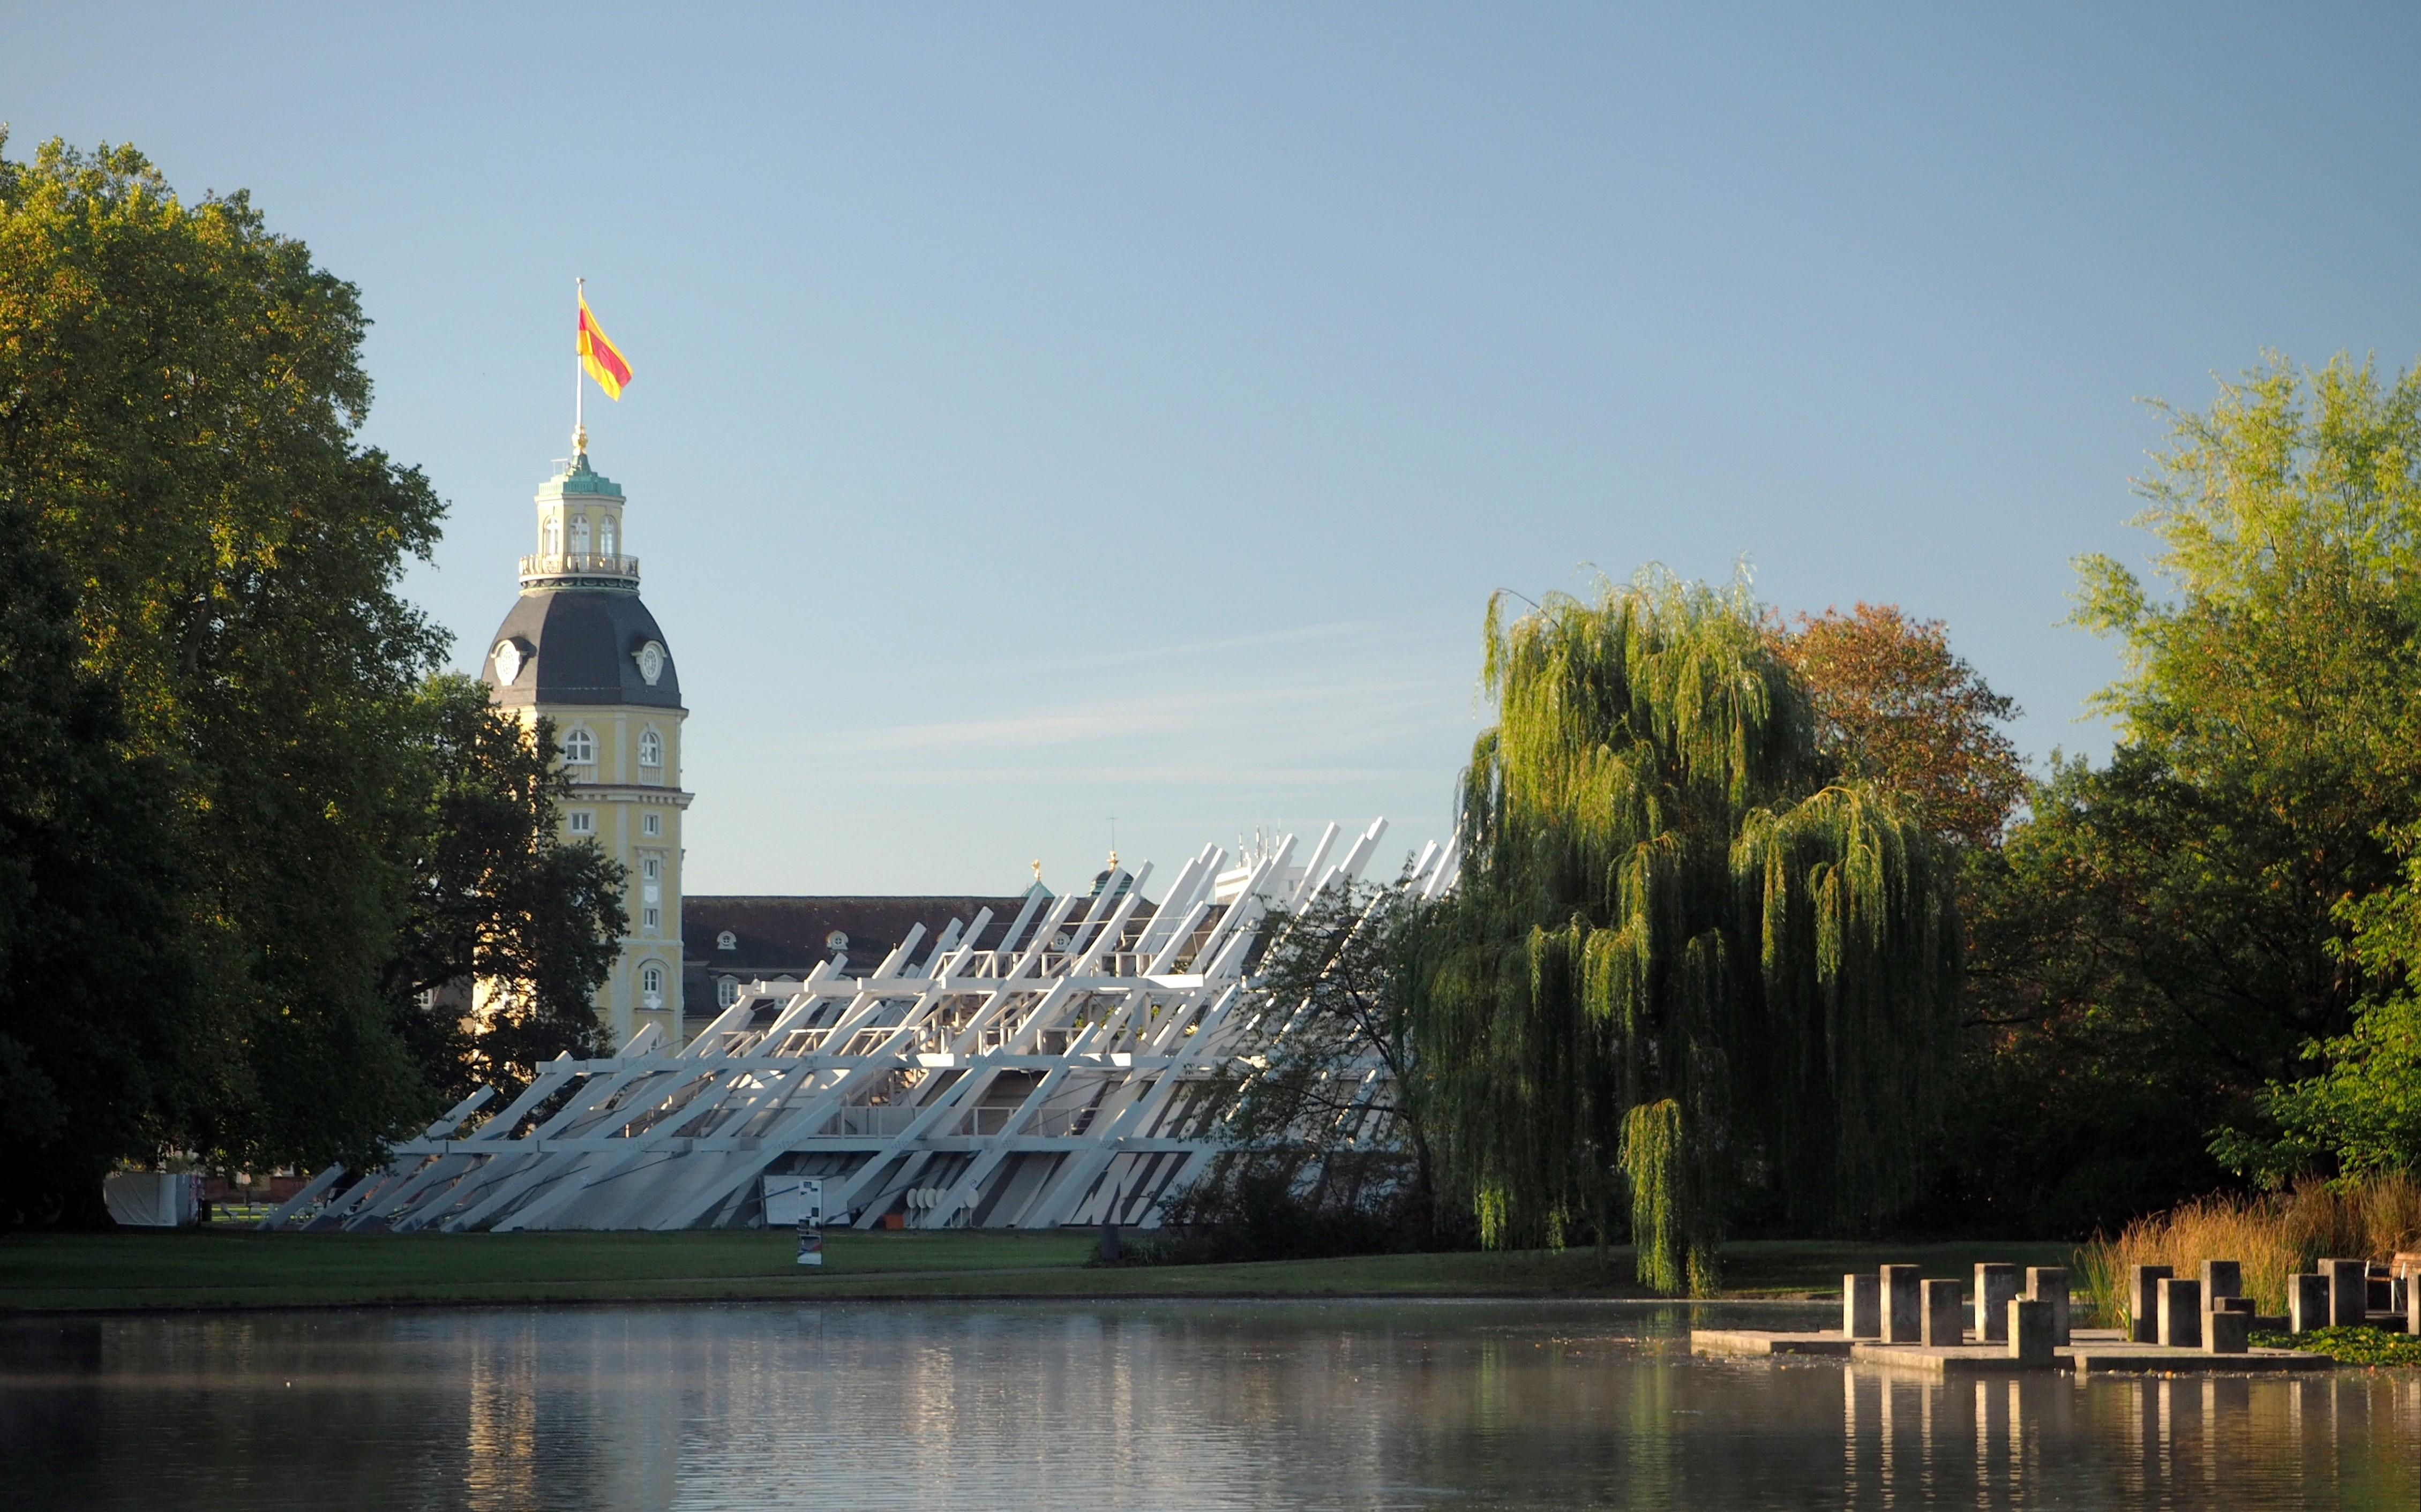
\includegraphics[width=21cm]{images/city/schlosspark-1.jpg}};
  \node[anchor=south west,color=white,outer sep=1ex] at (img.south west) {\imgtitle{Benjamin Berg}{Schlossteich and Schlossturm}{CC BY-SA 4.0}{}};
\end{tikzpicture}



\begin{tikzpicture}
\end{tikzpicture}

\vspace*{8.5cm}

\section{Concept and dates}

Our plan is to have the conference with two days on a weekend at the start to mid
August followed by three days for BoFs (Birds of a Feather). By having the core
days of the conference on the weekend we allow many people living close enough to visit
the conference without having to schedule their vacation around it. We are also
planning for the registration to be free and to finance the conference solely
using donations and corporate sponsorship.

In addition to the usual conference events we are planning to run an event
on Friday that is especially designed for students from the various universities
in Karlsruhe. We will give students a chance to learn more about free software,
the tools used, and how to contribute. For this event we are planning to collaborate with
OpenHatch\footnote{\url{http://openhatch.org}} as they have a lot of experience
with running these kind of events. With GUADEC right after these workshops
we give the students a unique chance to meet the community, learn more about GNOME,
and to start contributing.

\begin{tabularx}{\linewidth}{X|X|X|X|X|X}
\bf Friday & \bf Saturday & \bf Sunday & \bf Monday & \bf Tuesday & \bf Wednesday \\\hline
  pre-event \newline
  Registration \newline
  Social~Event
 &
  Core Day I \newline
  Social~Event
 &
  Core Day II \newline
  Social~Event
 &
  BoF I \newline
  ZKM tour \newline
  Social~Event
 &
  BoF II
 &
  BoF III
\end{tabularx}

\newpage

%\section{Dates}

%The traditional concept of two core days with keynotes and other 
%presentation, followed by a two-day hackfest was proven to be a winning 
%formula. We intend to keep those basics and add a little twist.

%We plan to run a pre-event on Friday, especially designed for 
%students in computer sciences degrees from the various universities in 
%Karlsruhe. The pre-event includes a general introduction to free and 
%open source software and a more specific overview over the GNOME 
%project and is followed by a few hands-on sessions. As two of the 
%members of the organizing team are teaching at DHBW, one of the 
%universities, we will be able to seamlessly integrate some particular 
%aspects of the GNOME projects with topics taught at university. 
%Ideally, we would like to involve our GSoC students as much as 
%possible, especially during the hands-on sessions, in order to lower 
%the initial barriers by creating a stimulating environment where the 
%students will feel that they are working with peers.

%\iffalse
%Furthermore, we plan to host the Sunday lecture session at ZKM, where 
%the end of the day can then be spent discovering the incredible variety 
%of art exhibitions and challenging each other at various games.
%\fi

%In summary, the event will be scheduled as follows:

%Friday:
%\begin{itemize}
%\item Pre-event for students
%\item Registration
%\item Social event at AKK or Z10
%\end{itemize}

%Saturday:
%\begin{itemize}
%\item  Core day I
%\item  Social event at XXX
%\end{itemize}

%Sunday:
%\begin{itemize}
%\item  Core day II at ZKM
%\item  AGM
%\item  GSoC Student Talks
%\end{itemize}

%Monday:
%\begin{itemize}
%\item  Hackfest day I
%\item  Visit of the Hoepfner Brewery
%\end{itemize}

%Tuesday 09.08.2016:
%\begin{itemize}
%\item  Hackfest day II
%\item  Picnic in the “Schlossgarten”
%\end{itemize}

